\documentclass[10pt,a4paper]{article}
\usepackage[utf8]{inputenc}
\usepackage[T1]{fontenc}
\IfFileExists{lmodern.sty}{\usepackage{lmodern}}{}
\usepackage[margin=1.8cm]{geometry}
\usepackage{amsmath,graphicx,booktabs,xcolor,enumitem}
\usepackage[most]{tcolorbox}
\graphicspath{{figures/}}
\setlist{itemsep=1pt,topsep=2pt,leftmargin=*}
\pagestyle{empty}
\newtcolorbox{qbox}[1][Questions]{colback=orange!8,colframe=orange!75!black,fonttitle=\bfseries,title={#1},
  left=4pt,right=4pt,top=2pt,bottom=2pt}
\newcommand{\sub}[1]{\par\smallskip\noindent\textbf{#1}\par}

\begin{document}
\begin{center}
{\Large\bfseries Gaussian Splatting for Physical Inverse Problems --- Meeting Brief}\\[2pt]
Muhammad Hussain Qureshi (MSDS25010) \quad·\quad Advisor: Dr.\ Ali Murtaza \quad·\quad 10 November 2026
\end{center}
\noindent\textbf{Core idea:} represent the unknown field as Gaussians, render them on a grid, and replace the camera
of Gaussian Splatting with the physics operator; fit to the measurements. Data from InverseBench.
\\ Code: \texttt{github.com/muhammadhussainqureshi/thesis-gs}

\section*{1.\ 3D Inverse Scattering}
\sub{What I did, and how}
\begin{itemize}
\item 3D Gaussians (position, scale, rotation, amplitude) reconstruct cell permittivity from scattered fields;
compared with a voxel grid optimised with the same loss.
\item \textbf{True 3D Born model} (your request): 3D Green's functions, 60 transmitters and 360 / 180 / 60 receivers
on a sphere. Verified against the exact point-scatterer response ($10^{-7}$).
\item Data: real 3D nuclei (BBBC024 / CytoPacq, $32\times128\times128$) and synthetic nuclei; also 2D InverseBench cells.
\item Fixes found along the way: a sparsity term (removes ``ghost'' copies in the sensors' blind spots) and a
\textbf{bounded density} $1-e^{-f}$ (Gaussians could overshoot; the grid is clipped to $[0,1]$).
\end{itemize}

\sub{Results (PSNR dB, true 3D model, same regularisation for both)}
\begin{center}
\begin{tabular}{lcccc}
\toprule
 & Parameters & 360 rec. & 180 rec. & 60 rec. \\
\midrule
Real nuclei: Gaussians (bounded) & 60k & \textbf{32.8} & \textbf{31.4} & \textbf{26.7} \\
Real nuclei: voxel grid & 524k & 32.5 & 30.5 & 25.6 \\
Synthetic: Gaussians (bounded) & 54k & \textbf{46.4} & \textbf{43.6} & \textbf{39.1} \\
Synthetic: voxel grid & 524k & 42.1 & 39.9 & 38.2 \\
\bottomrule
\end{tabular}
\end{center}
\begin{itemize}
\item Gaussians win on \textbf{every volume} at every receiver count, with \textbf{$\sim$9$\times$ fewer parameters}.
\item Without the bounded density they lost by 5--7\,dB. With more measurements (slice-wise 3D, 2D) the grid is
still slightly ahead (0.2--2.7\,dB).
\end{itemize}
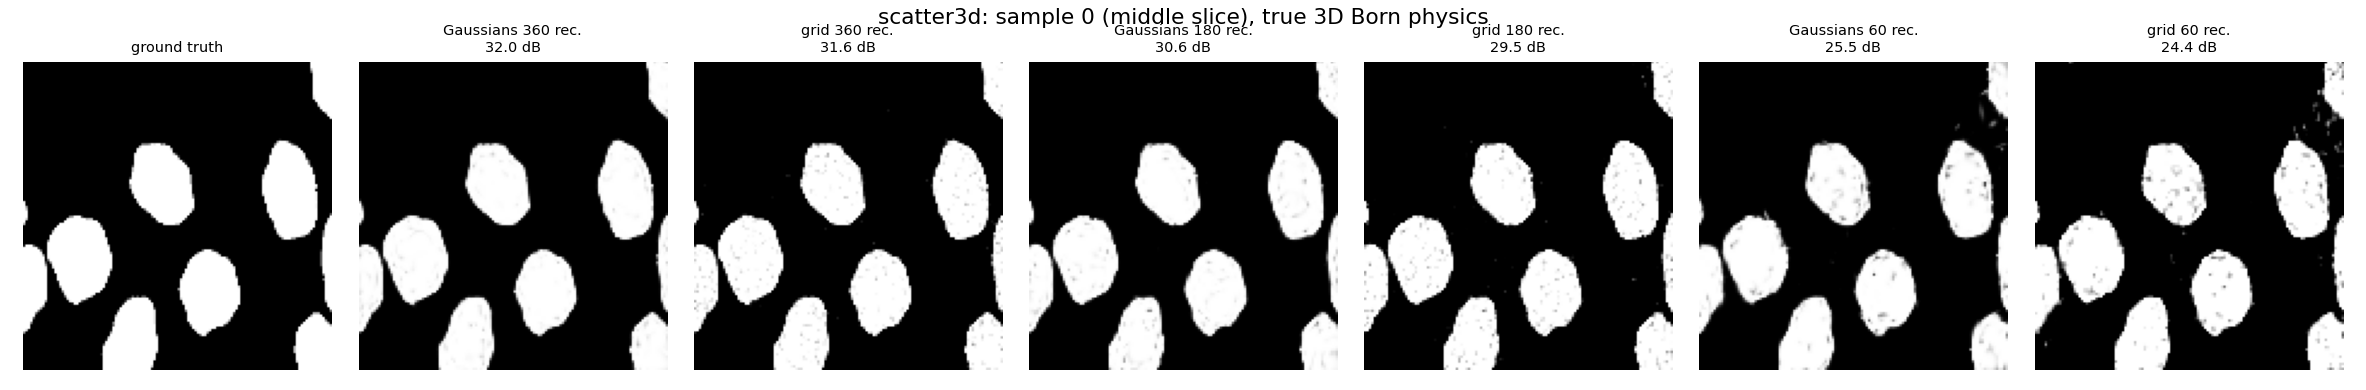
\includegraphics[width=\linewidth]{born3d_bbbc024_bounded.png}

\begin{qbox}
\begin{enumerate}
\item Is this true 3D (Born) model what you wanted? Is single scattering enough for Thesis I?
\item Can the claim be: \emph{bounded Gaussians are more accurate and $\sim$9$\times$ more compact when measurements
are scarce; a grid is better when data are plentiful}?
\end{enumerate}
\end{qbox}

\newpage
\section*{2.\ 4D Navier--Stokes}
\sub{What I did, and how}
\begin{itemize}
\item 4D Gaussians: canonical 2D Gaussians plus a \textbf{deformation network} that moves them over time
(2D + time, 21 frames, $Re=200$, InverseBench data).
\item Deformation by an \textbf{MLP} (as in 4D Gaussian Splatting) vs.\ \textbf{Mamba} (state-space model over each
Gaussian's trajectory) vs.\ static Gaussians; plus a temporal smoothness term.
\item Observed 100\% or only 10\% of pixels; 5 frames never observed (tested).
\end{itemize}

\sub{Results (PSNR dB on unseen frames, 3 flows)}
\noindent\begin{minipage}[t]{0.47\linewidth}\vspace{0pt}
\begin{tabular}{lccc}
\toprule
Observed & Static & MLP & Mamba \\
\midrule
100\% & 17.0 & \textbf{27.4} & 27.2 \\
10\% & 16.0 & 23.0 & \textbf{25.4} \\
\bottomrule
\end{tabular}
\begin{itemize}
\item Motion model: \textbf{+10\,dB} over static.
\item Sparse data: \textbf{Mamba +2.4\,dB} over MLP, on all 3 flows; MLP shows streaks.
\item Full data: equal. Mamba is $\sim$9$\times$ slower.
\end{itemize}
\end{minipage}\hfill
\begin{minipage}[t]{0.5\linewidth}\vspace{0pt}
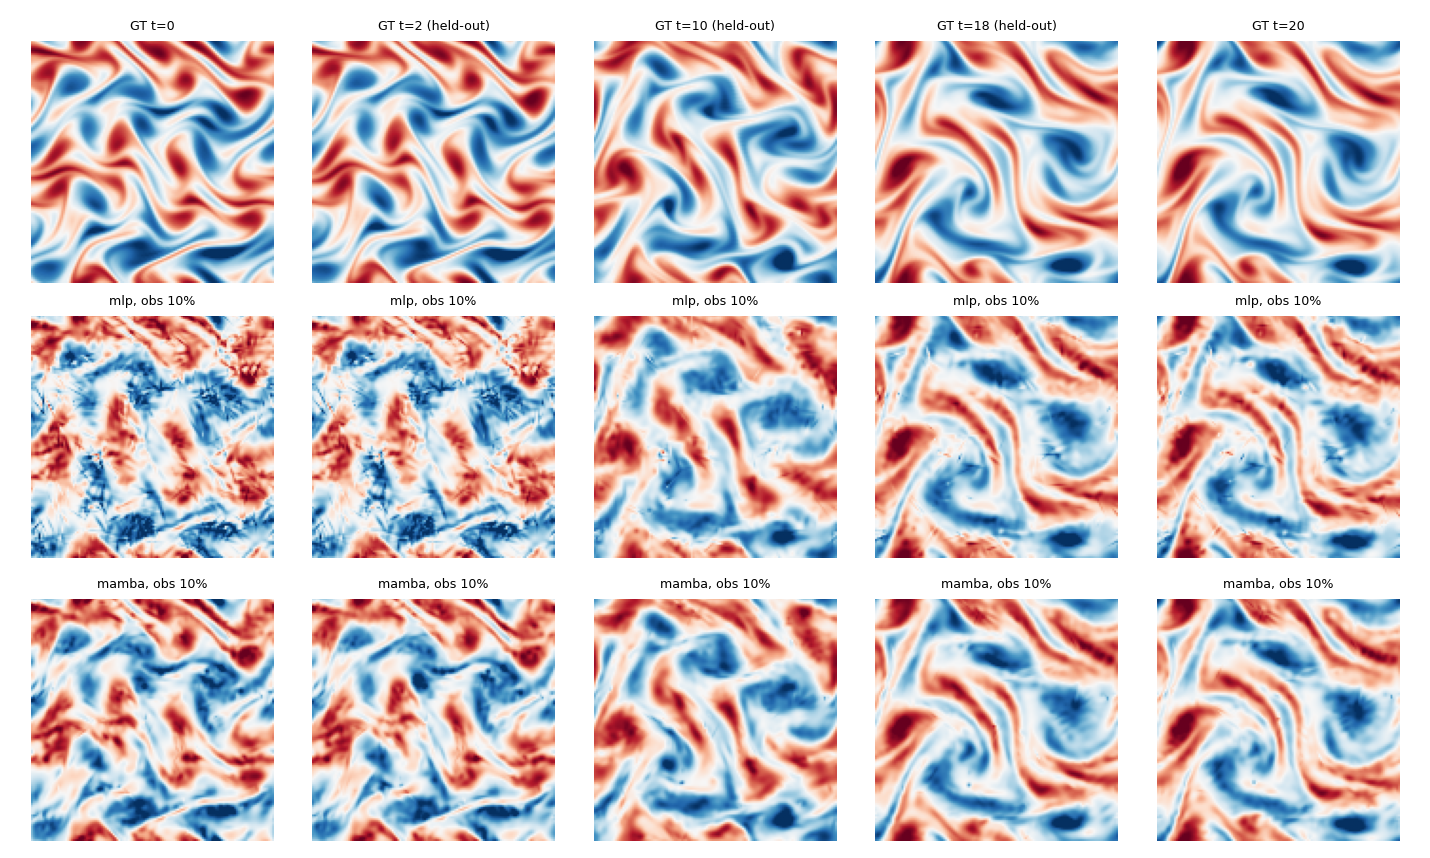
\includegraphics[width=\linewidth]{ns_sparse.png}\\
{\footnotesize Rows: truth, MLP, Mamba (10\% observed).}
\end{minipage}

\begin{qbox}
\begin{enumerate}\setcounter{enumi}{2}
\item Is reconstructing the flow from sparse observations acceptable, or should I add physics (Navier--Stokes
residual) or recover the initial condition through the solver, as InverseBench does?
\item Is Mamba as the motion model what you intended?
\end{enumerate}
\end{qbox}

\begin{qbox}[General questions]
\begin{enumerate}\setcounter{enumi}{4}
\item \textbf{Thesis I:} the exact list of targets, the required template, and the thesis title?
\item \textbf{Next 2 weeks:} physics-informed 4D model, more samples, or extending the literature review?
\end{enumerate}
\end{qbox}
\end{document}
